\section{Initial Dataset}

The social media exploited for this work is Twitter, a microblogging and social networking service where users post content and interact with posts known as “tweets”. Unlike other social platforms, Twitter allows to easily access published contents and to make complex queries to obtain filtered data.
The dataset has been obtained from Twitter thanks to a web-scraping phase using the snscrape library of Python specifying the following criteria: 
\begin{itemize}
\item \textbf{language}: italian. Has been taken into consideration only the italian tweets;
\item \textbf{date of posting}: tweets posted from 1st December 2021 to 1st February 2022; 
\item \textbf{specific keywords} contained into the text of the tweets: the keywords are separated by the or-operator and the set of keywords is composed by the most frequently body shaming used words;
\item \textbf{replies}, \textbf{quotes} and \textbf{retweet} have been discarded. 
\end{itemize}

\noindent
Applying these criteria 75,357 tweets have been collected.

\vspace{5mm}

\noindent
With a first cleaning step has been removed URLs, mentions, new lines and multiple spaces in order to simplify the subsequent manual labeling and, after that, tweets posted more than once from the same user or not containing none of keywords have been discarded obtaining a total of 59,583 tweets.

\vspace{5mm}

\noindent
The entire dataset has been divided in:
\begin{itemize}
    \item \textbf{training set}: December 2021 - January 2022
    \item \textbf{test set}: February 2022
\end{itemize}

\subsection{Training set}

From the 37,555 cleaned tweets of the period (1st December, 2021 - 31st January, 2022) some random tweets have been manually labeled with two possible class labels: body-shaming for the tweets with  negative physical comments, and non-body-shaming for the other tweets.
Every tweet has been read, interpreted and correctly class labeled; in this way have been found out:
\begin{itemize}
\item 788 tweets with body shaming label
\item 788 tweets with non-body shaming label
\end{itemize}
At the end, has been obtained an initial balanced dataset composed by 1576 tweets as shown in Figure \ref{classes} in which label '0' corresponds to the non-body-shaming tweets and label '1' to the body-shaming tweets. 


\begin{figure}[H]
    \centering
    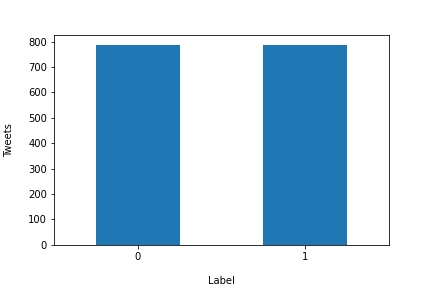
\includegraphics[width= 0.8\textwidth]{images/dataset/training set.png} 
    \caption{Labeled tweets of the training set} 
    \label{classes}
\end{figure}




